\section{Conception Détaillée}

\subsection{Extraction des étoiles et de leurs coordonnées}

\subsubsection{Objectifs}

L'Algorithme doit être capable de reconnaître une étoile puis de nous fournir ses coordonnées sur l'image.

\subsubsection{Etat de l'art}

Nous sommes dans un premier temps concentrés sur les différents algorithmes et méthodes déjà implémentées pour l'extraction d'étoiles et le traitement d'image.

\vspace{0.5cm}

\noindent \textbf{SIFT (Scale-Invariant Feature Transform)}\\
Méthode de détection et description de zones d’intérêt (features) où l’intensité lumineuse varie fortement. Le détecteur de Moravec analyse les variations d’intensité dans plusieurs directions autour d’un pixel. Une forte variation indique une feature, comme une étoile.

\vspace{0.5em}
\noindent \textbf{Top Hat pour l’extraction de points lumineux}\\
Transformation morphologique utilisée pour extraire de petits détails brillants :
\begin{itemize}[noitemsep]
    \item \textit{White top-hat} = image $-$ ouverture (isole les zones plus claires),
    \item \textit{Black top-hat} = fermeture $-$ image (isole les zones plus sombres).
\end{itemize}
Utilisée pour améliorer l’image ou corriger l’arrière-plan.

\vspace{0.5em}
\noindent \textbf{DAOStarFinder}\\
Algorithme de détection d’étoiles en trois étapes :
\begin{enumerate}[noitemsep]
    \item \textbf{Filtrage TopHat} : supprime le fond diffus pour isoler les objets brillants.
    \item \textbf{Détection de pics lumineux} : recherche les pics ressemblant à des étoiles, filtre le bruit.
    \item \textbf{Résultat} : liste d’étoiles avec coordonnées, brillance et taille.
\end{enumerate}

\subsubsection{Problèmes rencontrés et solutions choisies}

\begin{figure}[ht]
    \centering
    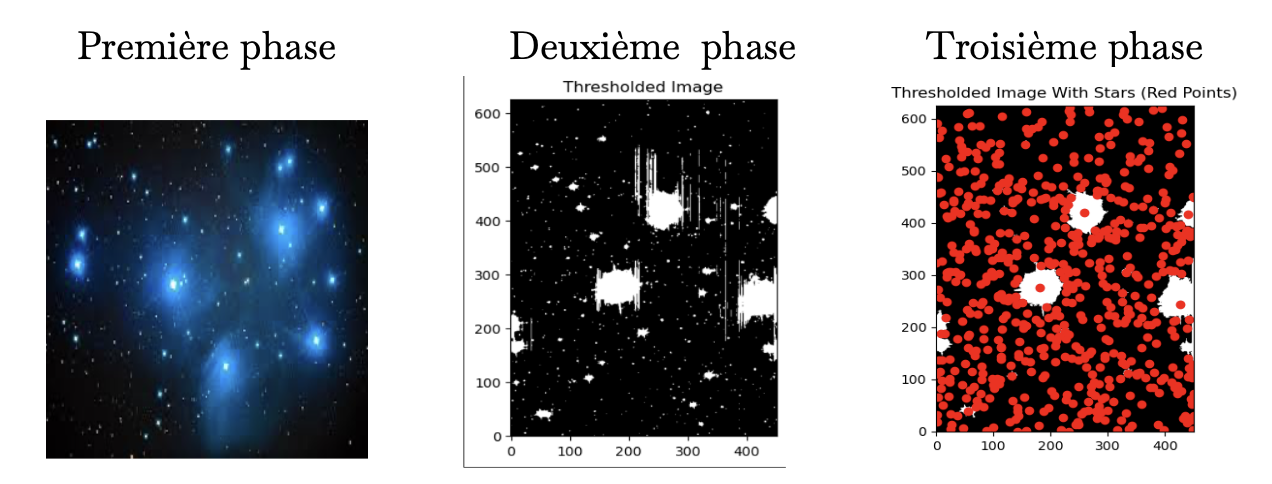
\includegraphics[width = 0.6\linewidth]{img/Topnaze.png}
    \caption{DAOstarfinder et étoiles avec halos étendus}
\end{figure}

Néanmoins, lorsque nous avons choisi la bibliothèque Python DAOStarFinder, nous nous sommes rendu compte qu’elle détectait \textbf{un trop grand nombre d’étoiles}, y compris des faux positifs. En effet, elle avait du mal à bien délimiter les contours, car certaines étoiles étaient \textbf{beaucoup plus lumineuses que d’autres}, ce qui créait des \textbf{halos plus étendus} autour d’elles et perturbait la détection. (Figure 6)

\vspace{0.3 cm}
\begin{figure}[ht]
    \centering
    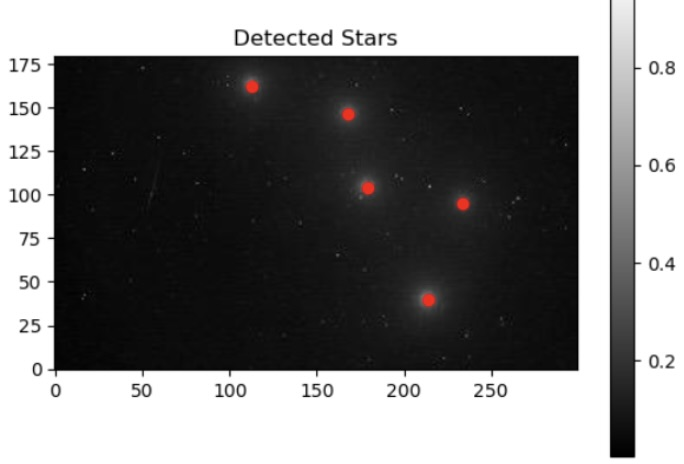
\includegraphics[width = 0.5\linewidth]{img/DAO.jpeg}
    \caption{DAOstarfinder avec étoiles bien définies}
\end{figure}

 \vspace{0.4cm}

\begin{figure}[ht]
    \centering
    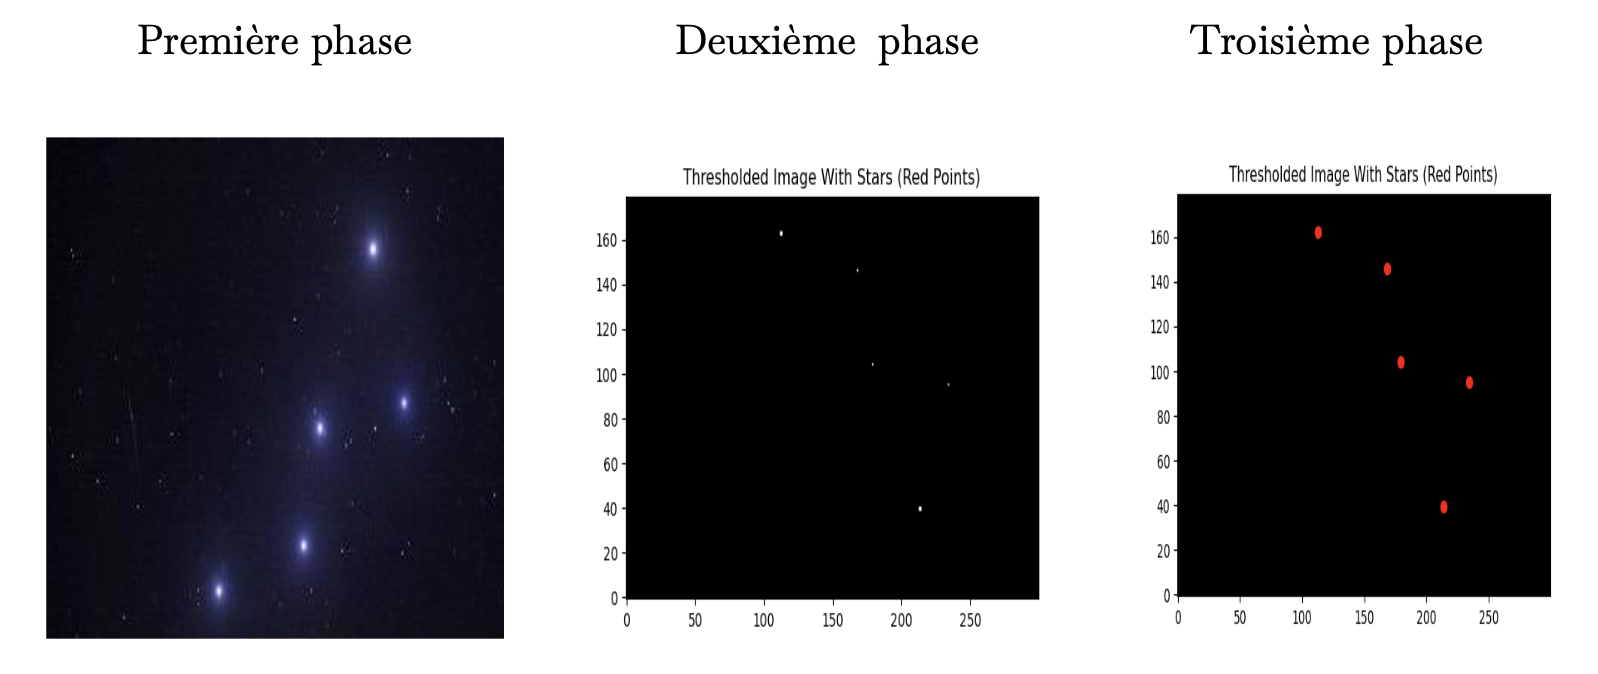
\includegraphics[width = 0.7\linewidth]{img/Topmarche.png}
    \caption{detection étoiles via notre méthode}
\end{figure}

 \vspace{0.3cm}

Dans le prolongement des difficultés précédemment rencontrées avec la détection d’étoiles, nous avons tiré parti de certaines fonctionnalités de la bibliothèque \textbf{DAOStarFinder}, en particulier du \textbf{seuil de détection} qu’elle génère par \textbf{indexation booléenne}.

 Nous avons ensuite développé un script permettant d’exploiter ce masque binaire afin d’identifier les zones lumineuses correspondant aux étoiles, ainsi qu’à leurs halos.

 Pour chaque forme détectée, nous avons calculé le \textbf{barycentre} afin d’estimer les \textbf{coordonnées centrales} de l’étoile associée.

À chaque étoile ainsi identifiée, nous avons attribué :

\begin{itemize}
    \item une \textbf{coordonnée} (déterminée à l’aide de notre propre méthode de calcul de barycentre),
    \item une \textbf{valeur de luminosité} (obtenue via la bibliothèque \textbf{Pillow}, en analysant l’intensité des pixels),
    \item et une \textbf{taille apparente}, estimée à l’aide d’un algorithme que nous avons conçu spécifiquement.
\end{itemize}

\newpage

\subsection{Correspondance des constellations avec la base de données}

\subsubsection{Objectifs}

Utiliser les propriétés d'invariance des constellations pour les différencier, Comparer les listes d'étoiles formées avec les constellations de la base de donnée avec une fonction de coût et Retourner le nom de la constellation correspondant le plus.

\subsubsection{Etat de l'art}
Pour la correspondance avec la base de données, la solution de l'IA étant trop nécessiteuse en données et pas forcément adaptée à notre cas, nous avons décidé de calculer une fonction de coût qui permet de distinguer les caractéristiques des constellations.

\vspace{0.5cm}

\noindent \textbf{ICP (Iterative Closest Point)}\\
Algorithme d’appariement de nuages de points :
\begin{enumerate}[noitemsep]
    \item Associe chaque point source à son plus proche voisin dans le nuage cible.
    \item Calcule la transformation (rotation + translation) minimisant la distance.
    \item Applique la transformation au nuage source.
    \item Répète jusqu’à convergence (écart minimal entre itérations).
\end{enumerate}

\vspace{0.4cm}

\noindent \textbf{Algorithme des Triangles similaires}

Compare des motifs géométriques formés par des groupes d'étoiles et exploite l'invariance des proportions des triangles.

\textbf{1. Triangulation} : On forme des triangles à partir des étoiles visibles dans l'image capturée (par exemple, à partir des plus brillantes).

\textbf{2. Caractérisation} : Chaque triangle est défini par des ratios de distances et ses angles.

\textbf{3. Base de données} : Ces caractéristiques sont comparées à une base de données contenant des triangles pré-calculés à partir de catalogues d'étoiles connues.

\textbf{4. Correspondance} : Si une correspondance est trouvée, elle minimise la fonction de coût du triangle.

\subsubsection{Problèmes rencontrés et solutions choisies}

3 questions essentielles se sont posées lors de notre réflexion sur la partie reconnaissance :

\begin{itemize}
    \item Quels critères pertinents utiliser pour distinguer deux constellations ?
    \item Aussi, comment comparer la liste d'étoiles de l'image avec les constellations de la base de donnée à partir de ces critères ? 
    \item Enfin, comment dessiner la constellation une fois la constellation identifiée ?
\end{itemize}

\vspace{0.2cm}

\noindent \textbf{Grandeurs invariantes d'un triangle, nos critères ?}

Puisque notre démarche de reconnaissance de constellation s'inspire de celle des astronomes, l'algorithme des triangles similaires était un choix qui nous a semblé judicieux. Les grandeurs propres et invariantes (par translation, rotation, changement d'échelle) d'un triangle sont notamment ses angles et ses rapports de longueur.

\vspace{0.4cm}

\noindent \textbf{Fonction de coût}

Nous avons choisi de normaliser la somme des rapports des côtés du triangle (rapports préalablement triés en amont entre les longueurs des côtés) et des angles de chaque triangle. En effet, les deux caractéristiques (rapports de longueurs et angles) ont la même importance donc nous leur attribuons un poids égal. Pour cela il faut les mettre au même ordre de grandeur (entre 0 et 1) d'où la normalisation.

\vspace{0.4cm}

\noindent \textbf{Détection des étoiles}

\vspace{0.2cm}

\noindent \textbf{1. Choix méthodologiques}

Le système de détection repose sur une approche simple mais plutôt robuste, visant à \textbf{extraire les étoiles les plus significatives} (les plus brillantes) d’une image astronomique. L’objectif est de réduire l’impact du bruit et de simplifier la correspondance avec les constellations.

\vspace{0.2cm}

\noindent \textbf{2. Méthodologie}

\noindent Extraction des étoiles brillantes :

Analyse de l’image pour détecter les sources lumineuses.
\textbf{Sélection des 20 étoiles les plus brillantes} qui est une instance de DetectedStarSet (luminosités comprises dans les informations fournies par le script Python dans le CSV).

\vspace{0.1cm}

\noindent Correspondance avec la constellation cible - Part I:

Pour chaque \textbf{\textit{Constellation}}, seules les 4 étoiles les plus brillantes qui correspondent le mieux à une certaine constellation sont retenues. Si la constellation possède plus d'étoiles, on calculera leur position avec de la géométrie (abordée plus tard).
Cette sélection diminue la fiabilité de la reconnaissance mais diminue de manière significative le temps de calcul.

\vspace{0.1cm}

\noindent Correspondance avec la constellation cible - Part II:

La fonction de coût est définie pour mesurer la proximité (géométrique et photométrique) entre ces 4 étoiles et un sous-ensemble équivalent parmi les étoiles détectées. On regarde toutes les combinaisons de 4 étoiles et nous conservons celle qui minimise le coût.

\vspace{0.1cm}

\noindent \textbf{3. Éléments majeurs du système}

\textbf{Star} : Représente une étoile individuelle avec ses coordonnées (x, y) dans l’image et sa brillance. C’est l’unité de base du traitement.

\textbf{StarSet} : Représente un ensemble d'étoiles composée de plusieurs étoiles. Permet de générer des triangles à partir des points.

\textbf{DetectedStarSet} : Représente une liste d'étoiles dans l'image à analyser. Cette classe permet notamment de générer des combinaisons d'étoiles et d'identifier l'ensemble d'étoiles correspondant le mieux à une constellation. Offre des méthodes qui forment des triangles et extraient des sous-ensembles candidats.

\textbf{Triangle} : Représente un triplet d’étoiles. Chaque triangle est caractérisé par ses longueurs de côtés et ses angles internes. Il sert à comparer des structures stellaires (patrons) entre l’image et les constellations.

\textbf{Constellation} : Contient une description d’un groupe d’étoiles connues. Inclut un nom, une liste d'adjacence qui représente schématiquement les liaisons entre étoiles et de la même façon que DetectedStarSet, on peut calculer les triangles formés par les étoiles principales.

\noindent \textbf{4. Problème d'hypothèse et de complexité}

L'hypothèse initiale pour le calcul du coût des triangles : l'ordre des étoiles est conservé pour un même set d'étoiles par rapport à celui de la base de données. Seulement, cette hypothèse n'est pas toujours respectée lorsque l'on fournit une image différente de la même constellation qui a permis de faire la base de données et les coûts calculés sont donc faux. Il faudrait donc maintenant itérer sur toutes les permutations d'étoiles. D'où le problème de complexité.

\vspace{0.4cm}

L'extraction des étoiles nous permet de ranger les étoiles d'une images dans leur ordre de brillance.

\begin{figure}[ht]
    \centering
    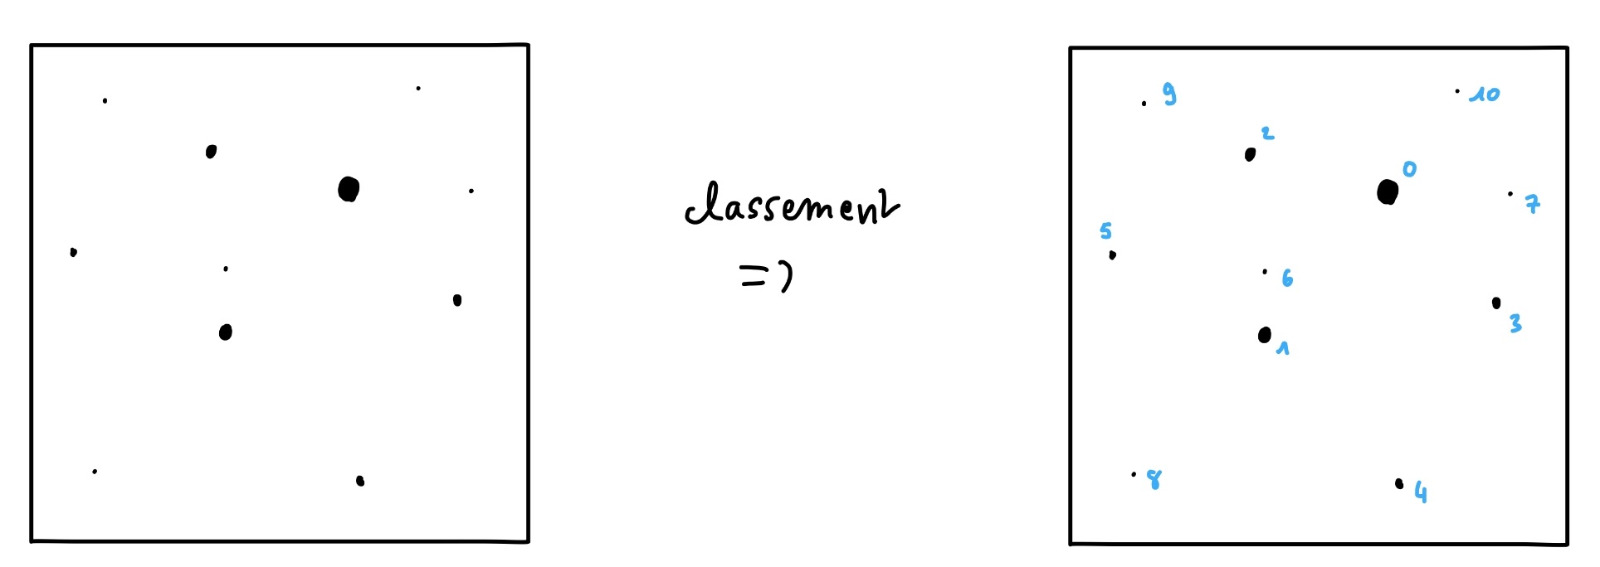
\includegraphics[width = 0.7\linewidth]{img/Pb1.jpeg}
    \caption{Exemple de classement}
\end{figure}

Par exemple, à gauche on a une image à analyser avec des étoiles, après extraction, on peut numéroter les étoiles en fonction de leur brillance (figure de droite). Ainsi, nous avions au début fait l'hypothèse que ce classement était toujours le même, quelle
que soit la manière dont on prenait en photo une constellation. Cette hypothèse nous simplifiait grandement le calcul de la correspondance entre une constellation et un set de d'étoiles.
Malheureusement, après de nombreux tests, nous nous sommes rendus compte qu'elle était
dans beaucoup de cas pas vérifiée.

\begin{figure}[ht]
    \centering
    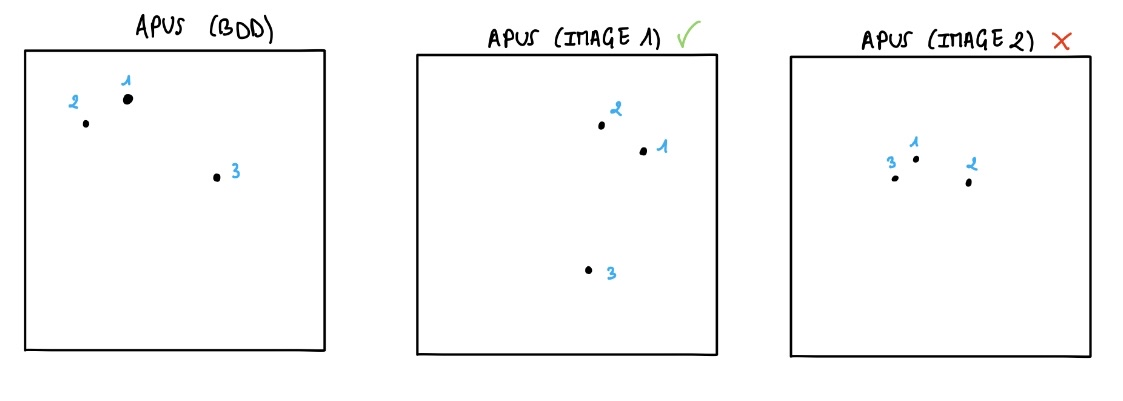
\includegraphics[width = 0.7\linewidth]{img/Pb2.jpeg}
    \caption{Exemple de contracdiction de l'hypothèse}
\end{figure}

Voici un exemple avec la constellation Apus. Sur la gauche, on observe la constellation telle qu'elle a été considérée dans la base de données. Au milieu, une image de la même
constellation prise à un autre moment, où les étoiles ont été extraites et où la condition est vérifiée. Enfin, sur la droite, une image où la condition n'est pas vérifiée.
Dans le cas où les rangs ne sont pas conservés, le coût entre la constellation et le set d'étoiles
sera faussé.

\begin{figure}[ht]
    \centering
    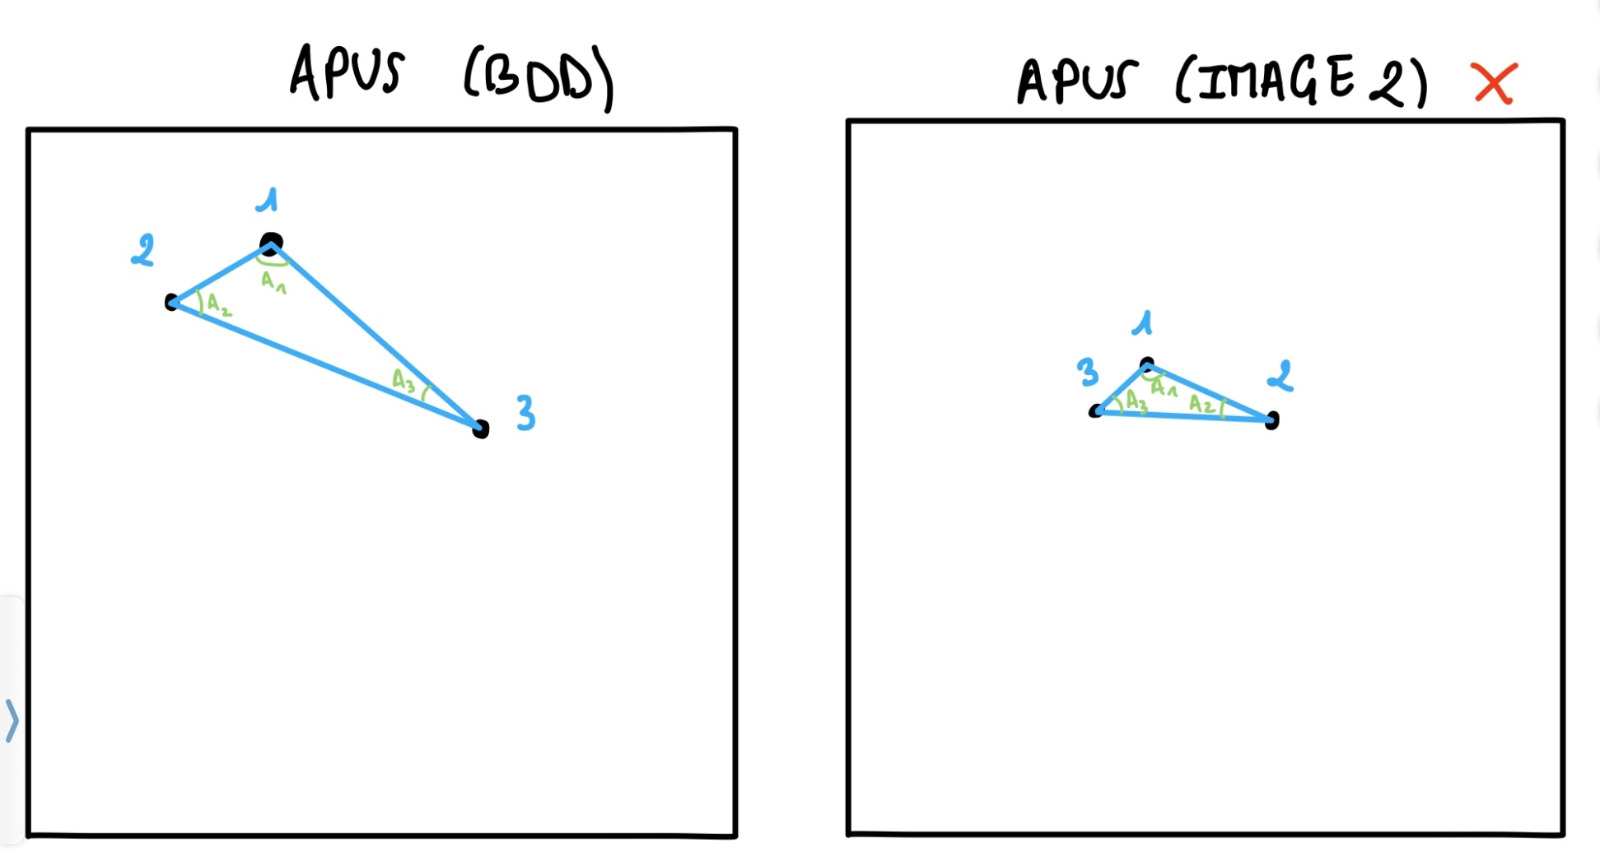
\includegraphics[width = 0.7\linewidth]{img/Pb3.jpeg}
    \caption{Exemple de cas où le coût est anormalement élevé pour la même constellation}
\end{figure}

En reprenant l'exemple précédent, on observe que les angles 2 et 3 ne correspondent pas. (On peut faire la même conclusion pour les longueurs normalisées) Cela va donc provoquer un grand coût, alors que c'est la bonne constellation. Il y aura donc des erreurs de
reconnaissance.
Ainsi, nous avons abandonné cette hypothèse. Mais cela signifiait qu'il fallait énumérer toutes les possibilités de rangs entre les étoiles et choisir uniquement celle qui minimisait le coût.
Notre algorithme présentait déjà des temps de calculs significatifs (autours de la minute), et ce changement de paradigme a amplifié ce phénomène.
Après réflexion, nous nous sommes tournées vers la solution suivante :
Plutôt que de minimiser le coût entre un ensemble complet d’étoiles et une constellation, nous avons restreint notre recherche à la comparaison entre tous les groupes de 4 étoiles de l’image et les 4 étoiles les plus brillantes de chaque constellation. Une fois la meilleure correspondance identifiée, nous avons utilisé des propriétés géométriques en particulier les angles et les positions relatives pour localiser les autres étoiles de la constellation sur l’image.

\subsection{Interface}
\subsubsection{Objectifs}
Réaliser une interface qui lorsqu'on lui donne une image du ciel nous renvoie la constellation associée si une constellation est présente.

\subsubsection{Etat de l'art}

Dans le développement d’interfaces graphiques en Java, deux bibliothèques principales coexistent : \textbf{Java Swing} et \textbf{JavaFX}.

\begin{itemize}
    \item \textbf{Java Swing}

 Swing a longtemps été la bibliothèque standard pour créer des interfaces graphiques en Java. Elle offre une large panoplie de composants (boutons, fenêtres, menus...) et repose sur le concept de \textbf{modèles de rendu léger}. Cependant, \textbf{Swing est aujourd’hui considéré comme obsolète} pour plusieurs raisons :
    \begin{itemize}
        \item Son architecture est datée, moins réactive et peu adaptée aux applications modernes riches en interactions et animations.
        \item Le design des composants est rigide et difficile à personnaliser sans manipulations complexes.
        \item Elle n’est plus activement développée : bien qu'encore maintenue, elle n’évolue plus vraiment.
    \end{itemize}
    \item \textbf{JavaFX}

 JavaFX est le successeur officiel de Swing. Il a été conçu pour répondre aux \textbf{besoins des interfaces modernes} : plus dynamiques, plus fluides, et plus esthétiques. JavaFX apporte plusieurs avantages notables :
    \begin{itemize}
        \item \textbf{Gestion améliorée des événements} et du \textbf{multimédia} (audio, vidéo, animations).
        \item Meilleure intégration des \textbf{effets graphiques}, des \textbf{animations}, et des \textbf{styles CSS}.
        \item Possibilité de créer des interfaces plus réactives, évolutives, et orientées utilisateur.
        \item Il prend également en charge des outils de conception visuelle comme \textbf{Scene Builder}.
    \end{itemize}
\end{itemize}

\paragraph{\textbf{Pourquoi nous avons choisi JavaFX}}

Le choix de \textbf{JavaFX} s’est imposé naturellement dans le cadre de notre projet. Notre interface nécessitait :

\begin{itemize}
    \item une \textbf{grande flexibilité graphique} (pour afficher des éléments dynamiques comme la rose des vents, les points lumineux, etc.),
    \item une \textbf{gestion fluide des événements} (animations, interactions utilisateur)


\end{itemize}
JavaFX s’est révélé plus adapté que Swing sur tous ces points, en particulier grâce à son \textbf{système de scène}, sa prise en charge native des \textbf{transitions animées}, et sa capacité à \textbf{lier dynamiquement les propriétés} des composants à des données ou à des calculs.



\subsubsection{Problèmes rencontrés et solutions choisies}

Au début de notre développement, nous avons opté pour \textbf{Scene Builder} afin de faciliter la création de notre interface. Cependant, après plusieurs essais, nous avons constaté que la \textbf{prise en main} s'est révélée plus complexe que prévu, notamment quand il s’agissait de placer correctement les éléments sur la scène. En effet, certains boutons ne s’affichaient pas à l’emplacement souhaité une fois le programme lancé.
 
Nous avons donc pris la décision de \textbf{ne pas utiliser Scene Builder} et de passer directement par un fichier \textbf{FXML} pour définir la structure de notre interface, et un fichier \textbf{CSS} pour styliser les composants. Cette approche a été plus \textbf{simple} à maîtriser, mais elle a tout de même présenté des \textbf{difficultés}.
 
En particulier, la gestion du placement des éléments s'est avérée délicate : les composants \textbf{s'influencaient les uns les autres} (notamment avec les \textbf{layouts} comme \verb|VBox| ou \verb|HBox|), ce qui a rendu complexe le positionnement précis des éléments. De plus, l’\textbf{ordre des éléments dans le fichier FXML} a joué un rôle crucial, car il affectait leur positionnement et leur affichage à l'écran.

De plus, il est important de noter que \textbf{JavaFX} n’est pas entièrement compatible avec certaines propriétés du \textbf{CSS}, ce qui a compliqué la personnalisation de certains éléments visuels. En particulier, pour le \textbf{loader} que nous voulions intégrer, il a été nécessaire de \textbf{créer une classe Java dédiée} pour implémenter sa fonctionnalité et son animation, car les styles CSS ne permettaient pas de réaliser cette animation complexe.

